\documentclass{pre-tfg}

% \showhelp  % comenta o borra para eliminar ayudas

\title{Desarrollo de aplicaciones móviles con tecnologías híbridas para gestionar el proceso de ideación en las organizaciones}
\author{Eduardo Parra Mazuecos}
\advisorFirst{Javier Bustamante Pérez}
\advisorDepartment{DEPARTAMENTO DE TECNOLOGÍAS Y SISTEMAS DE INFORMACIÓN}
\advisorSecond{Manuel Ángel Serrano Martín}
\intensification{INGENIERÍA DEL SOFTWARE}
\docdate{2018}{Junio}


\begin{document}

    \maketitle
    \tableofcontents

    \newpage

    \section{INTRODUCCIÓN}

    Nextinit~\cite{NEXT} es una plataforma para la gestión del proceso de ideación que potencia la innovación desde
    abajo hacia arriba, dentro de la organización, transmitiendo cualquier idea de un miembro de la organización a
    cualquier posición de esta.

    Las ideas se crean dentro de la plataforma como si fueran startup que necesitan dinero para empezar. Los usuarios,
    además de poder crear ideas, pueden invertir dinero virtual en ellas para aumentar el capital de la idea para que
    esta puede llevarse a cabo. Cuando una idea recibe mucha inversión por parte del resto de usuarios significa que 
    los personas de esa organización creen que es una buena idea.
    
    Como cada usuario tiene dinero limitado, estos no pueden invertir a todas las ideas porque si la idea no sale adelante,
    pierden el dinero. En cambio, si la idea se lleva a cabo recuperan el dinero invertido, además de unos intereses.

    La forma de dar a conocer y aplicar la idea en la organización es la siguiente:
    \begin{enumerate}
        \item Un miembro de la organización crea la idea en Nextinit, aportando un capital semilla a su elección.
        \item Se inicia la búsqueda de fondos para soportar la idea, donde cada miembro de la organización puede
        aportar el capital que desee.
        \item Si alcanza el mínimo de capital se considera la idea como soportada, pero se puede seguir invirtiendo
        capital hasta que termine el periodo de financiación.
        \item El siguiente paso es que la empresa apruebe la idea.
        \item Si se ha aprobado la idea se lanza un proyecto piloto.
        \item Una vez que se ha probado el piloto se implementa la idea en la organización.
    \end{enumerate}

    Actualmente Nextinit tiene un gran problema con las aplicaciones móviles, ha cambiado con frecuencia el equipo de
    desarrollo, la complejidad del código es elevada, las aplicaciones utilizan librerías de terceros que han sido
    abandonadas, la aplicación es poco robusta y el coste de realizar cambios es elevado.

    Se estudió la posibilidad de desarrollar dos nuevas aplicaciones nativas, tanto para Android~\cite{NEXTAN} como
    para IOS~\cite{NEXTIP}, pero hubieran sido dos desarrollos distintos, con el consecuente aumento de coste y tiempo.

    En este proyecto se realizará un único desarrollo para crear las dos aplicaciones móviles, mejorando el
    funcionamiento respecto a las antiguas versiones y añadiendo nuevas funcionalidades de las que no dispone
    actualmente.
    
    
     \begin{picture}(0,0)
		 \put(0,-120){
    	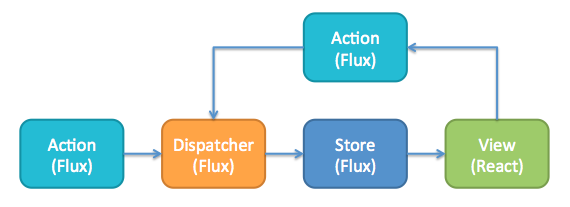
\includegraphics[height=4.8cm]{flux.png}}
    \end{picture}
     
     \singlespacing
     \singlespacing
     \singlespacing
     \singlespacing
     \singlespacing
     \singlespacing
     \singlespacing
     \singlespacing
     
	\textit{Esquema de la arquitectura Flux con React Native y Redux utilizada en el proyecto~\cite{FLUXIMG}}
	\singlespacing
	\singlespacing
    \section{TECNOLOGÍA ESPECÍFICA / INTENSIFICACIÓN / ITINERARIO CURSADO POR EL ALUMNO}

    \begin{table}[hp]
        \centering
        \caption{Tecnología Específica cursada por el alumno}
        \label{tab:tec-especifica}

        \zebrarows{1}
        \begin{tabular}{p{0.1\linewidth}p{0.4\linewidth}}
            & \textbf{Marcar la tecnología cursada} \\
            \hline
            & Tecnologías de la Información \\
            & Computación \\
            X & Ingeniería del Software \\
            & Ingeniería de Computadores \\
            \hline
        \end{tabular}
    \end{table}


    %  \clearpage


    \begin{table}[hp]
        \centering
        \caption{Justificación de las competencias específicas abordadas en el TFG}
        \label{tab:competencias}

        \zebrarows{1}
        \begin{tabular}{p{0.5\linewidth}p{0.4\linewidth}}
            \textbf{Competencia} & \textbf{Justificación} \\
            \hline
            Capacidad para desarrollar, mantener y evaluar servicios y sistemas software que satisfagan
            todos los requisitos del usuario y se comporten de forma fiable y eficiente, sean asequibles
            de desarrollar y mantener y cumplan normas de calidad, aplicando las teorías, principios,
            métodos y prácticas de la Ingeniería del Software.
            & El software del proyecto se desarrollará usando la arquitectura Flux~\cite{FLUX} para el manejo
             y flujo de datos, y se utilizarán los principios  y buenas practicas de Ingeniería del Software, 
             como la utilización de metodologías ágiles y tecnologías para la mejora de la calidad.\\
            Capacidad para valorar las necesidades del cliente y especificar los requisitos software para
            satisfacer estas necesidades, reconciliando objetivos en conflicto mediante la búsqueda de
            compromisos aceptables dentro de las limitaciones derivadas del coste, del tiempo, de la existencia
            de sistemas ya desarrollados y de las propias organizaciones.
            & El proyecto requiere de unos requisitos flexibles, que pueden ser modificados a lo largo del
            desarrollo. Los requisitos se recogerán y validarán en las reuniones periódicas de seguimiento
            del desarrollo con las personas responsables de la empresa.\\
            Capacidad de dar solución a problemas de integración en función de las estrategias, estándares
            y tecnologías disponibles.
            & La aplicación resultante debe conectarse con una API REST para almacenar y obtener información
            necesaria de la base de datos.\\
            Capacidad de identificar y analizar problemas y diseñar, desarrollar, implementar, verificar y
            documentar soluciones software sobre la base de un conocimiento adecuado de las teorías, modelos
            y técnicas actuales.
            & Se analizará el cumplimiento del desarrollo, de acuerdo a la metodología. Los problemas o
            decisiones que se tomen durante el trascurso del proyecto serán documentadas de tal forma que
            pueda entenderse lo ocurrido correctamente. \\
            Capacidad de identificar, evaluar y gestionar los riesgos potenciales asociados que pudieran presentarse.
            & Para prevenir posibles riesgos, se comprobará con una lista con los riesgos mas comunes en proyectos
            software y se estudiará el impacto en el proyecto. \\
            Capacidad para diseñar soluciones apropiadas en uno o más dominios de aplicación utilizando métodos
            de la ingeniería del software que integren aspectos éticos, sociales, legales y económicos.
            & Se velará el correcto cumplimiento de la LOPD~\cite{LOPD}, gestionando correctamente los datos de los
            usuarios y de las empresas.\\
            \hline
        \end{tabular}
    \end{table}

	\clearpage

    \section{OBJETIVOS}

    El objetivo principal de este TFG es la creación de una aplicación para móviles para utilizar la plataforma 
    Nextinit anteriormente descrita, desarrollada con tecnologías híbridas que permita con un único 
    desarrollo, funcionar en IOS y Android, adaptándose de forma adecuada a cada sistema operativo. La 
    aplicación móvil será creada desde cero, se integrará mediante una API REST con la aplicación web de 
    Nextinit. Se incluirá la funcionalidad disponible en la anterior aplicación móvil de Nextinit, además, de otras 
    funcionalidades nuevas.
    \newline\newline
    Para conseguir la finalidad principal de este TFG, se deben cumplir los siguientes objetivos:
    \begin{enumerate}
        \item Crear un sistema para autenticarse con los credenciales de la plataforma o a través de 
        la intranet de un cliente de Intelygenz en concreto.
        \item Mejorar la experiencia de usuario en las aplicaciones móviles de Nextinit, creando una aplicación 
        intuitiva y fácil de usar.
        \item Obtener unas aplicaciones móviles más robustas que las que había anteriormente, a las que
        poder añadir nuevas funcionalidades con mayor rapidez y facilidad.
        \item Crear una aplicación que solo incorpore las funcionalidades que más se usaban de las aplicaciones
        antiguas y añadir otras nuevas.
    \end{enumerate}


    \section{MÉTODO Y FASES DE TRABAJO}

    Para el desarrollo se usará una metodología basada en eXtreme Programming~\cite{XP} adaptada para
    adecuarla a un equipo con un solo desarrollador.
    Se ha elegido esta metodología porque es adecuada para un equipo pequeño y con requisitos
    muy cambiantes.


    Principios fundamentales~\cite{XPAGIL} de los 12 de eXtreme Programming, que se pondrán en práctica:
    \begin{enumerate}
        \item Planificación incremental - La planificación es iterativa, el cliente elige al comienzo de cada
        iteración que historias de usuario se van a implementar.
        \item Releases pequeñas - Se liberan versiones iterativas con mucha frecuencia, en máximo una o dos semanas.
        La versión liberada debe estar preparada para implementarse en producción, es decisión de el cliente hacerlo
        o no.
        \item Uso de metáforas - El diseño debe de ser fácil de explicar a personas nuevas en el proyecto. Por eso,
        se deben nombrar los objetos con nombres con los que personas sin conocimientos puedan identificarlos.
        \item Simplicidad en el diseño - El diseño debe ser sencillo, si hay código complejo se debe reemplazar
        por otro sencillo. Para considerar que el código es sencillo, debe ser sencillo de testear, de comprender,
        de encontrar el código buscado y de explicar.
        \item Testing - Los test son esenciales, es necesario crear test unitarios y de aceptación, estos últimos
        son ideados por el cliente. Los test se escriben antes de desarrollar el código.
        \item Refactorización de código - Se realiza durante todo el ciclo de vida del proyecto, ahorra tiempo
        y aumenta la calidad.
        \item Integración continua - El código debe integrarse en el repositorio cada pocas horas y siempre se debe
        trabajar con la última versión.
        \item 40 horas semanales - Se debe trabajar a un ritmo que se pueda mantener indefinidamente, sin días muertos,
        sin tareas que realizar, ni exceso de horas. Un trabajador cansado rinde menos, por lo que no se deberían
        superar las 40 horas de trabajo a la semana.
        \item El cliente es parte del equipo - Existe una persona representante del cliente en el equipo. Esta persona
        está disponible en todo momento para resolver dudas y decidir que se hace en cada momento.
        \item Estándares de codificación - El estilo de codificación debe ser consistente para que se encuentre en
        buen estado y otras personas sepan modificar cualquier parte del código.
    \end{enumerate}

    Ciclo de vida del proyecto~\cite{XPKENT}:
    \begin{enumerate}
        \item Exploración - El cliente escribe las historias de usuario, mientras el desarrollador se familiariza
        con las herramientas y la tecnología que se usarán en el proyecto.
        \item Planificación - El cliente establece la prioridad de cada historia de usuario, se acuerdan las historias
        de la entrega y se establece un cronograma. El desarrollador estima el esfuerzo de la implementación de las
        historias. Se lleva un registro de los puntos obtenidos en cada iteración, los cuales son la suma de los puntos
        de todas las historias de usuario realizadas en la iteración. Esos puntos de iteración o puntos de velocidad
        se usa para determinar cuántas historias de usuario se pueden realizar en una iteración.
        \item Iteraciones - Esta fase incluye varias iteraciones del proyecto. En la primera iteración se suele
        establecer una arquitectura que utilizar durante el resto del proyecto y en la última se debe tener un sistema
        listo para lanzarlo a producción. En el plan de elaboración se tiene en cuenta las historias de usuario
        no realizadas, los puntos de las iteraciones, y las tareas sin acabar de la iteración anterior.
        \item Producción - Esta fase requiere de pruebas extras y revisiones del sistema antes de que
        este sea llevado a producción. En este punto, todavía pueden tomarse decisiones sobre las características
        que incorporará la release actual.
        \item Mantenimiento - Mientras la versión anterior está en producción, el equipo debe mantener el sistema
        en funcionamiento mientras desarrolla la siguiente versión.
    \end{enumerate}


    \section{MEDIOS QUE SE PRETENDEN UTILIZAR}

    \subsection{Medios Hardware}

    Para la realización de este TFG se utilizará un ordenador, un móvil Android y un iPhone.
    El equipo necesario ha sido facilitado por Intelygenz.
    \begin{itemize}
        \item \textbf{MacBook Pro} Procesador Intel Core i5 @2.5GHz. 8GB RAM 1600 MHz. macOS High Sierra v10.13.5
        \item \textbf{Nexus 5x} Procesador Qualcomm® Snapdragon™ 808 64 bits, 1.8 GHz, seis núcleos, 2GB RAM con Android 8.1
        \item \textbf{iPhone 8} Procesador Apple A10 Fusion Quad-Core 64 bits, 2.23 GHz, 2GB RAM con IOS 11
    \end{itemize}

    \subsection{Medios Software}

    El software necesario para la realización del proyecto es el siguiente:
    \begin{itemize}
        \item Android Studio~\cite{ASTUDIO}, para desarrollar la parte nativa de Android de la aplicación.
        \item ECMAScript~\cite{ECMA}~\cite{ECMABOOK}, es el lenguaje en el que se realiza el desarrollo.
        \item IntelliJ IDEA Community~\cite{IDEA}, para desarrollar la mayor parte de la aplicación.
        \item React Native~\cite{RENA}~\cite{REACTBOOK}, es el framework que se usa para realizar el desarrollo.
        \item Redux~\cite{REDUX}, para desacoplar el estado global en React Native utilizando el patrón Flux.
        \item Redux Thunk~\cite{THUNK}, es un middleware que se usará para disparar acciones de redux.
        \item Jest~\cite{JEST}, se utilizará para realizar tests unitarios a la aplicación.
        \item Native Base~\cite{NABA}, se utilizará para realizar el estilo visual de la aplicación.
        \item Standard~\cite{STAND}, se usará como guía de estilo del código.
        \item Xcode~\cite{XCODE}, para desarrollar la parte nativa de IOS de la aplicación.
    \end{itemize}


    \section{REFERENCIAS}

    \bibliographystyle{alpha}
    \singlespacing
    \bibliography{main}

    \section{CONTRATO DE PROPIEDAD INTELECTUAL}

    Proyecto desarrollado en base a una colaboración entre la empresa Desarrollos informáticos Intelygenz S.L. y
    la Escuela Superior de Informática (ESI) de Ciudad Real, bajo el convenio FORTE. Todo posible software desarrollado
    derivado de dicha colaboración será propiedad exclusivamente de Desarrollos informáticos Intelygenz S.L, pudiendo ser
    utilizado sin excepción alguna con fines comerciales. De igual manera, todo beneficio económico derivable de su venta,
    uso o explotación, será únicamente un derecho de Desarrollos informáticos Intelygenz S.L.

\end{document}


% Local Variables:
% coding: utf-8
% mode: flyspell
% ispell-local-dictionary: "castellano8"
% mode: latex
% End:
